\documentclass[12pt,a4paper,titlepage]{article}
\usepackage[utf8]{inputenc}
\usepackage[finnish]{babel}
\usepackage{setspace}
\usepackage{parskip}
\usepackage{amssymb}
\usepackage{amsmath}
\usepackage{graphicx}
\usepackage{fancyhdr}
\usepackage[top=1in, bottom=1in, left=1in, right=1in]{geometry}
\usepackage{float}
\usepackage[section]{placeins}
%\usepackage[numbered,autolinebreaks,useliterate]{mcode} % jos tahdot laittaa matlabkoodia näkyville niin kannattaa käyttää tätä

% hyödyllisiä paketteja:
\usepackage{siunitx}\sisetup{per=frac} % SI-yksiköitä.
%\usepackage{supertabular} % jos tarttee isoja taulukoita
%\usepackage{fullpage} % pienemmät marginaalit jos haluaa

\usepackage{hyperref} % lisääthän omat pakettisi ENNEN hyperref'iä
\hypersetup{pdfborder={0 0 0}}
\onehalfspacing
\cfoot{}
\rhead{\thepage}
% asettaa nyk. kappaleen nimen vasempaan ylänurkkaan, saa poistaa jos haluaa
\lhead{\leftmark}

%%%%% kaikki ennen tätä liittyy käytettäviin paketteihin tai dokumentin muotoiluun. siihen ei tarvinne aluksi koskea. %%%%%

% prosenttimerkillä alkavat rivit ovat kommentteja: niitä ei katsota dokumenttia käännettäessä eli ne ovat vain kirjoittajaa varten

%%%%%%%%%%%%%%% Oleellinen sisältö alkaa%%%%%%%%%%%%%%%
\begin{document}
\section{SURF}
Kokeilin viittä kuvaparia, joista neljä esitti samaa henkilöä tai kohdetta. Ensimmäisenä kokeilin kuvaparia, jossa oli Sarah Jessica Parker ja hevonen. Tästä parista SURF löysi ainoastaan yhden vastaavuuden, mikä on luontevaa, koska kuvat eivät ole samasta kohteesta. Yhteneväisyydet ovat nähtävissä kuvassa \ref{parker}.

\begin{figure}
\centering 
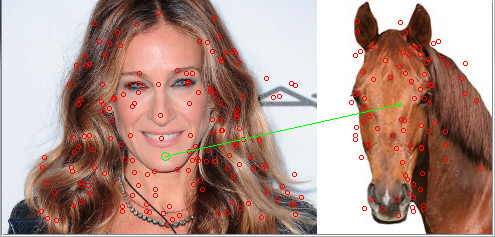
\includegraphics[width=\textwidth]{kuvat/sarahhorse.jpg}
\caption{Sarah Jessica Parker ja hevonen.}
\label{parker}
\end{figure}

Seuraavaksi kokeilin kuvaa kahdesta tähtitieteen professori Friedrich William August Argelanderia esittävästä maalauksesta. Näistä maalauksista SURF löysi neljä yhtäläisyyttä, joista kuitenkin vain kaksi oli todellisia (nenänpieli ja hiusraja ohimolla). Nämä ovat nähtävissä kuvassa \ref{argelander}. Jostain syystä Argelanderin hiuksien ja taustan välinen rajapinta tunnistettiin kuitenkin liiviksi kahdessa pisteessä.

\begin{figure}
\centering 
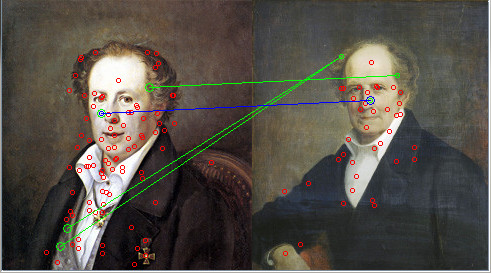
\includegraphics[width=\textwidth]{kuvat/argelander.jpg}
\caption{Kaksi maalausta professori Argelanderista.}
\label{argelander}
\end{figure}

Seuraavaksi kokeilin kahta valokuvaa samasta henkilöstä. Henkilöksi valitsin Heikki Ojan. Hänen kuvissaan havaitut kaksi yhtäläisyyttä ovat nähtävillä kuvassa \ref{heikkiseta}. Molemmat löydettiin samalta alueelta ylähuulen yläpuolelta, mikä on kiinnostavaa, koska kohdassa on vain tasaista ihoa. Toisaalta lähialueella on paljon helposti tunnistettavalta vaikuttavia muotoja (nenä, huuli, posken ryppy).

\begin{figure}
\centering 
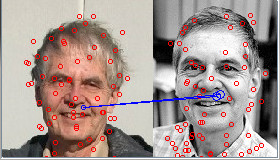
\includegraphics[width=\textwidth]{kuvat/heikkiseta.jpg}
\caption{Kaksi kuvaa Heikki Ojasta.}
\label{heikkiseta}
\end{figure}

Näiden henkilökuvien jälkeen siirryin rakennuksiin. Ensimmäisenä kokeilin Kaivopuiston tähtitornia, jonka arvelin helpoksi tunnistettavasti myös eri suunnista, sillä rakennus on melko symmetrinen. Kuvista löytyi viisi yhteyttä, joista ainoastaan kolme on todellisia toisiaan vastaavia piirteitä (nähtävillä kuvassa \ref{kaivopuisto}). Todellisten yhteyksien lisäksi esimerkiksi aurinkokellon vieressä oleva kivi oli yhdistetty pilveen. SURF tunnisti kuitenkin onnistuneesti avoimen ja suljetun kuvun samaksi objektiksi.

\begin{figure}
\centering 
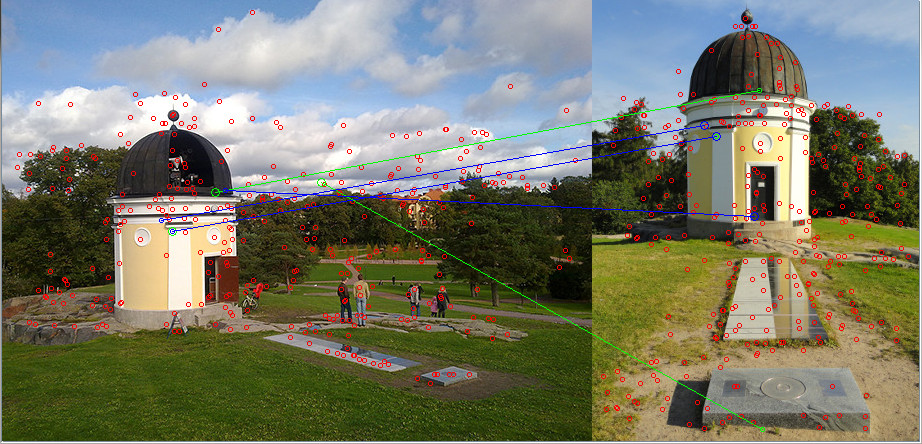
\includegraphics[width=\textwidth]{kuvat/kaivopuisto.jpg}
\caption{Kaivopuiston tähtitorni kahdesta suunnasta.}
\label{kaivopuisto}
\end{figure}

Toiseksi tutkittavaksi rakennukseksi valitsin Helsingin Observatorion (kuva \ref{obsis}). Kuvien valaistusolosuhteet poikkeavat toisistaan melko paljon, mutta kuvakulmat ovat lähellä toisiaan. SURF vaikuttaa kuitenkin keskittyneen yhtäläisyyksien etsimisessä rakennusta enemmän läheisiin puihin, joista on vaikea sanoa, ovatko yhdistetyt piirteet todella samoja. Kuuden seitsemästä yhteydestä voidaan kuitenkin suoralta kädeltä sanoa olevan virheellisiä, sillä niissä on yhdistetty rakennuksen osia puihin.

\begin{figure}
\centering 
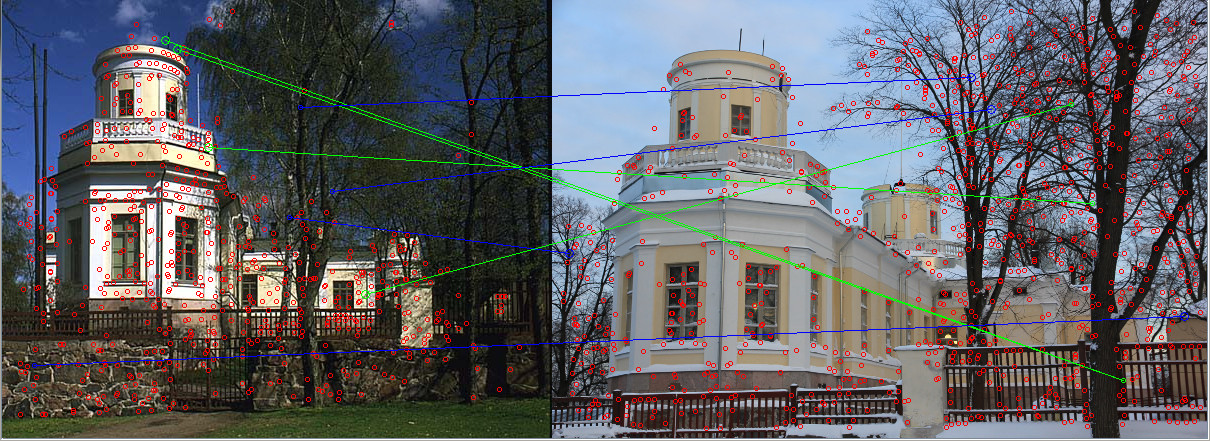
\includegraphics[width=\textwidth]{kuvat/obsis.jpg}
\caption{Helsingin Observatorion länsipääty kahtena eri vuodenaikana.}
\label{obsis}
\end{figure}

Viimeksi kokeilin kahta melko paljon toisiaan muistuttavaa kaavakuvaa Aurinkokunnan planeetoista (kuva \ref{aurinkokunta}). Niiden väliltä löytyi kuusi yhteyttä, joista kaikki paitsi Neptunuksen lähelle piirretty yhteys yhdistävät ihmissilmään sangen erilaisilta näyttäviä alueita.

\begin{figure}
\centering 
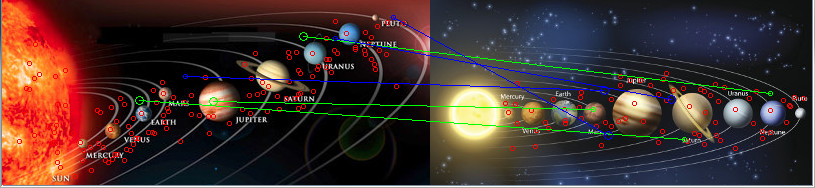
\includegraphics[width=\textwidth]{kuvat/aurinkokunta.jpg}
\caption{Kaksi kaavakuvaa Aurinkokunnan planeetoista.}
\label{aurinkokunta}
\end{figure}

Edellisten kuvien vastaavuuksia on tunnistettu melko heikosti. Etsiessäni hyvin toimivaa kuvaa löysin kaksi kuvaa Star Trekin Mr. Spockista käsi vulkaanitervehdykseen nostettuna. Näiden kuvien väliltä SURF löysi 13 yhteyttä, joista kaikki paitsi kaksi (päälaki yhdistetty olkapäähän) ovat todellisuudessa toisiaan vastaavien kohtien välillä. Yhteydet ovat nähtävissä kuvassa \ref{spock}. Kuvien välillä muuttuva rajaus ei vaikuta hämäävän ohjelmaa.

\begin{figure}
\centering 
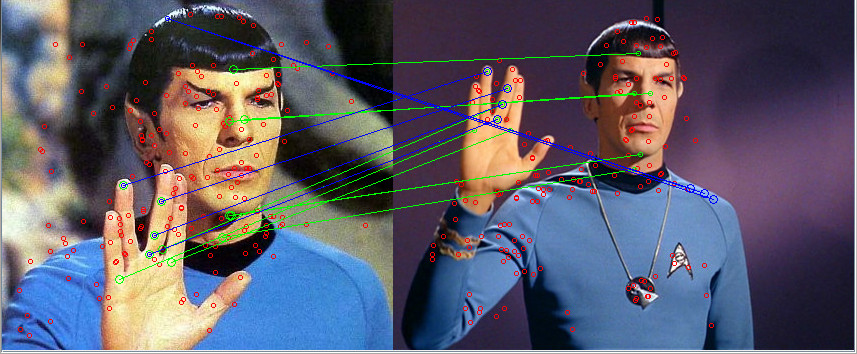
\includegraphics[width=\textwidth]{kuvat/spock.jpg}
\caption{Mr. Spock samassa asennossa.}
\label{spock}
\end{figure}

Tutkiakseni kuvanmuokkausten vaikutusta SURF:n kykyyn löytää yhtäläisyyksiä, valitsin kuvan astronautista ja tein sille useita erilaisia muokkauksia. Näistä ensimmäinen, gaussian blur, on nähtävissä ylimpänä kuvassa \ref{nautit}. Kuten kuvasta nähdään, kuvan terävyyden vähentämisestä huolimatta yhtäläisyyksiä löydetään melko paljon. Samassa kuvassa ovat nähtävissä myös kohinan lisäämisen, vääristämisen, kääntämisen ja väritasapainon säätämisen jälkeen saatavat yhteydet. Näiden perusteella nähdään, että ainoastaan sumentaminen vähentää merkittävästi yhteyksien määrää.

\begin{figure}
\centering 
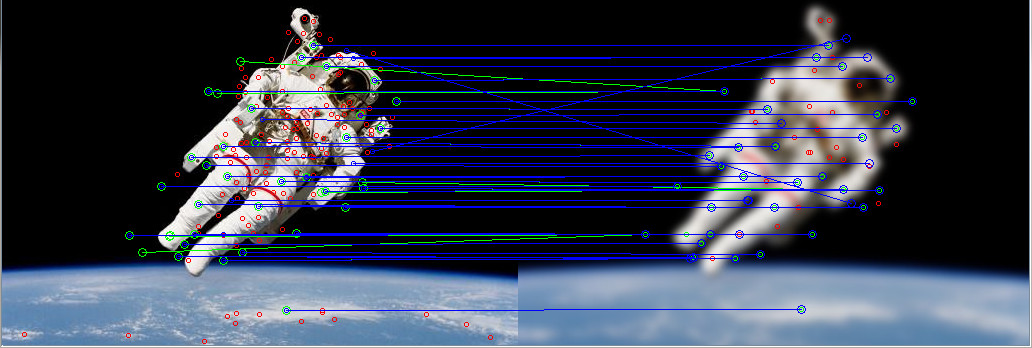
\includegraphics[width=0.8\textwidth]{kuvat/blurnautti.jpg}
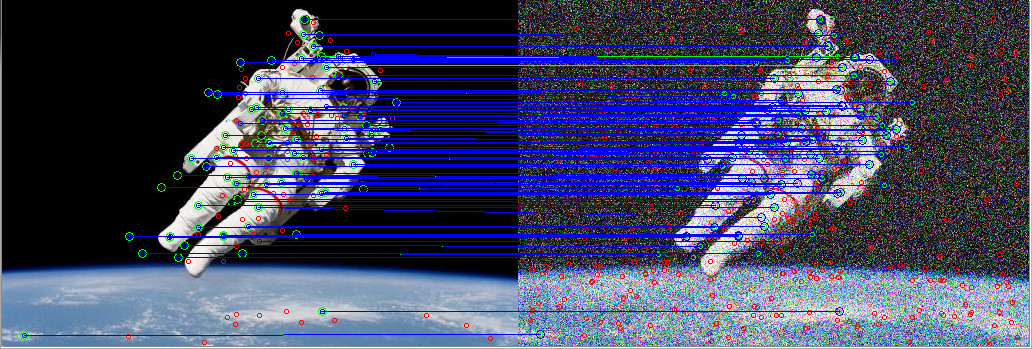
\includegraphics[width=0.8\textwidth]{kuvat/noise.jpg}
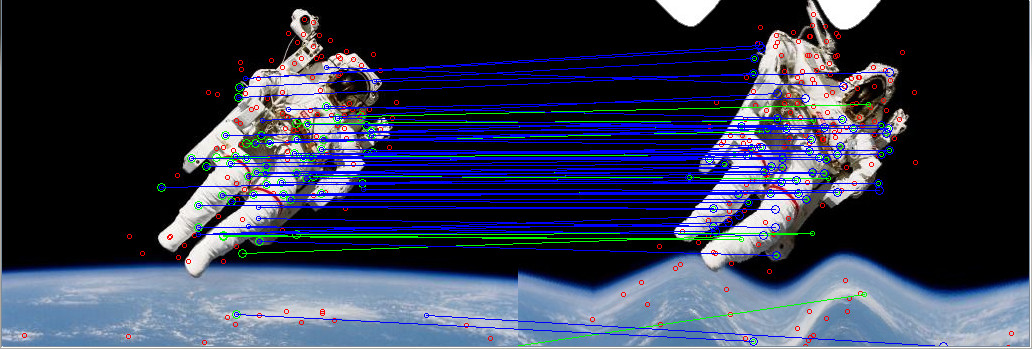
\includegraphics[width=0.8\textwidth]{kuvat/vaaristys.jpg}
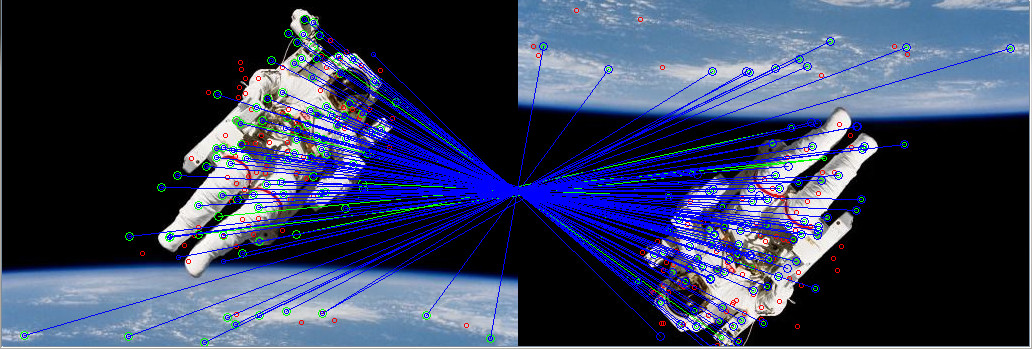
\includegraphics[width=0.8\textwidth]{kuvat/kaanto.jpg}
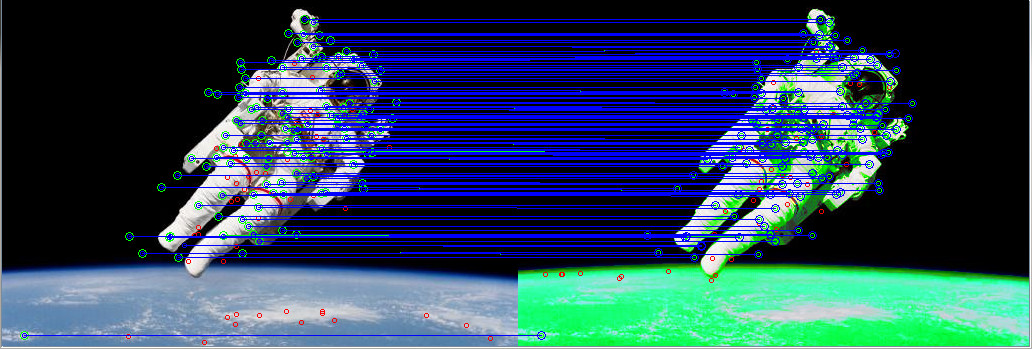
\includegraphics[width=0.8\textwidth]{kuvat/vari.jpg}
\caption{Kuva astronautista verrattuna sumennettuun, kohinaiseen, vääristettyyn, käännettyyn ja väritasapainoltaan muutettuun kuvaan.}
\label{nautit}
\end{figure}

\end{document}
